\documentclass{article}

% Support both uploading this folder alone and selecting this file as the
% main document when the parent repository is uploaded to Overleaf.
\newif\ifcompiledfromparent
\IfFileExists{workshop/neurips_2026.sty}{\compiledfromparenttrue}{\compiledfromparentfalse}
\ifcompiledfromparent
  \makeatletter
  \def\input@path{{workshop/}}
  \makeatother
\fi

\usepackage[dblblindworkshop]{neurips_2026}
\workshoptitle{LPFM}

\usepackage[T1]{fontenc}
\usepackage[utf8]{inputenc}
\usepackage{microtype}
\usepackage{inconsolata}
\usepackage{graphicx}
\ifcompiledfromparent\graphicspath{{workshop/}}\fi
\usepackage{booktabs}
\usepackage{amsmath}
\usepackage{amssymb}
\usepackage{multirow}
\usepackage{needspace}
\usepackage{nicefrac}
\usepackage{xcolor}
\usepackage{hyperref}
\usepackage{url}

\title{Decoding and Steering Graded Causal Implication in Pretrained Language Models}

\author{Anonymous Author(s)}

\begin{document}
\maketitle

\begin{abstract}
We study whether pretrained language models behaviorally register graded causal implication, whether that information is linearly accessible, whether representational evidence tracks graded judgments, and whether predictable decision failures can be reduced by activation steering. Across seven models, critical items produce both greater surprisal for a subsequent claim of causal ignorance and a larger factor-probability advantage after \emph{because} than after an explicit happenstance continuation. Direct Yes/No and Likert judgments are more mixed: two Qwen models are highly discriminative, while several other models exhibit weak thresholded accuracy and strong order sensitivity. Across six models, causal probes and contrastive activation addition (CAA) directions discriminate held-out causal items well, whereas directions trained on temporal contrasts transfer inconsistently. Representational scores correlate strongly with an external Gemini rating but, for several models, only weakly with the model's own prompted judgments. Development-selected raw activation interventions improve held-out balanced accuracy in several settings. These results distinguish behavioral sensitivity, linear accessibility, and final decision readout.
\end{abstract}

\section{Introduction}
\label{sec:introduction}

When one event is described immediately after another, comprehenders often infer more than temporal succession: the first event may be understood as explaining why the second occurred. This graded causal implication supports ordinary narrative understanding, explanation, and commonsense reasoning. A language model that is sensitive to the distinction should separate genuinely explanatory factors from details that are merely compatible with an event. Yet a model's prompted answer need not transparently reveal whether it represents that distinction. Answer-token priors, scale presentation, and late-stage readout can all distort an otherwise informative internal signal.

This representation--behavior distinction parallels recent work on event plausibility. Lepori et al. show that linear directions in language-model activations can distinguish modal categories and align with fine-grained human judgments even when output probabilities provide an unreliable behavioral measure \citep{lepori2026fantasy}. Causal implication presents a related but more relational problem: the model must evaluate whether a stated factor explains a particular event, rather than assess the plausibility of one sentence in isolation. Temporal proximity is a particularly important alternative explanation because causes normally precede their effects, but temporal order alone does not establish an explanatory relation.

Before asking how causal implication is represented, we first test whether it is visible in unconstrained next-token behavior. Following the ignorance-continuation logic of \citet{pan-kehler-2025-pragmatic}, an inferred explanation should make a subsequent claim that the reason is unknown less expected. A complementary diagnostic compares the probability of the same factor after \emph{because} versus after the explicitly incidental continuation \emph{and it so happened that}. Together, these tests avoid requiring the model to interpret a metalinguistic Yes/No question or numeric scale.

We therefore analyze causal implication at four levels. First, we compare implicit eliciture signatures from the ignorance and explicit-happenstance diagnostics with direct probabilistic Yes/No and Likert judgments. Second, we compare prompted behavior with linear probes and paired mean-difference directions, and test whether causal and temporal representations transfer across domains. Third, we ask whether the resulting continuous representation scores track probabilistic Yes/No judgments, probabilistic Likert judgments, and an external graded rating. Fourth, we distinguish two probe-relative decision failures: \emph{suppression}, in which the causal probe decodes a factor as explanatory but the model rejects it, and \emph{post-hoc attribution}, in which the probe decodes a factor as non-explanatory but the model accepts it. We test whether these failures are predictable from pre-answer activations and whether subtracting development-selected failure directions changes the final decision.

Our experiments are organized around the following research questions:

\begin{samepage}
\noindent\textbf{RQ1: Behavioral eliciture diagnostics.} Do causal critical items, relative to matched controls, increase the surprisal of a subsequent ignorance claim and increase the probability of the explanatory factor after \emph{because} relative to \emph{and it so happened that}? How consistently does this implicit sensitivity appear in direct probabilistic Yes/No and Likert judgments?
\end{samepage}

\begin{samepage}
\noindent\textbf{RQ2: Decodability and transfer.} Is graded causal implication linearly decodable across pretrained model families, and is the decoded causal signal distinct from a direction learned for temporal relations? How does internal decodability compare with prompted Yes/No and Likert behavior?
\end{samepage}

\begin{samepage}
\noindent\textbf{RQ3: Correlation with graded judgments.} Do raw causal probe logits and CAA projections track item-level graded judgments from the target model and an external rater, both across individual items and in critical-minus-control pair differences?
\end{samepage}

\Needspace{6\baselineskip}
\begin{samepage}
\noindent\textbf{RQ4: Predicting and reducing failure modes.} Can probe-relative suppression and post-hoc attribution be predicted from pre-answer activations and reduced by format-balanced, development-selected residual-stream steering without substantially damaging probe--output agreements?
\end{samepage}

\section{Methods}
\label{sec:methods}

\subsection{Models}
The RQ1 continuation diagnostics evaluate seven pretrained, non-instruction-tuned autoregressive language models: Gemma 2 2B and 9B, Qwen3 4B and 8B, Llama 3 8B, Llama 3.2 3B, and OLMo 3 7B. The direct prompted judgments and RQ2--RQ4 use the same set except OLMo 3 7B. For representation analyses, we use the residual stream at the final prompt token. Computation uses bfloat16 model weights; extracted activations and fitted analysis objects are stored with fixed dataset and checkpoint hashes.

\subsection{Data}
The main causal training and development sets contain 2,000 rows (1,000 critical--control pairs) and 400 rows (200 pairs), respectively. The held-out causal evaluation set contains 300 rows (150 pairs). Within a pair, the critical item supports the target event as a causal consequence of the stated factor, whereas the control preserves the event and discourse structure while adding a non-explanatory factor. The revised training and development files are \texttt{rc\_modifier\_train\_set.txt} and \texttt{rc\_modifier\_dev\_set.txt}; these historical filenames contain the revised independent-clause stimuli used in this analysis. Held-out items are distinct from training and development items.

For the temporal ablation, we use 800 training, 200 development, and 200 test pairs. Positive and negative temporal items contrast an event-consistent temporal relation with a matched non-temporal control. The causal and temporal data are fit independently; cross-domain evaluations apply a frozen probe or direction from one domain to the other.

\subsection{RQ1: behavioral eliciture diagnostics}
RQ1 uses the 300 held-out causal rows (150 matched critical--control pairs), equally divided between relative-clause and modifier constructions. Scores use raw, untempered next-token log probabilities. For the ignorance diagnostic \citep{pan-kehler-2025-pragmatic}, we remove the context's terminal period and append the exact continuation ``\texttt{, and I don't know why.}'' The row score is the negative summed log probability of all continuation tokens,
\begin{equation}
 I_i=-\log P(\text{\emph{and I don't know why}}\mid x_i),
\end{equation}
so a positive critical-minus-control gap indicates that professing ignorance is less compatible with the inferred explanation in the critical item.

For the explicit-happenstance diagnostic, let $E_i$ be the event and $F_i$ the factor. Let $B_i$ denote the reconstruction prefix ending in $E_i$ followed by \emph{because}, and let $S_i$ denote the matched prefix ending in $E_i$ followed by \emph{and it so happened that}. We score the identical factor tokens after these prefixes and compute
\begin{equation}
 H_i=\overline{\log P}(F_i\mid B_i)-\overline{\log P}(F_i\mid S_i).
\end{equation}
The mean over factor tokens prevents target length from determining the score. A positive critical-minus-control gap means that causal framing provides a larger relative advantage for explanatory than irrelevant factors. RQ1 does not use the separate \emph{because}--versus--bare-\emph{and} diagnostic.

For each measure, we report critical and control means, the matched critical-minus-control gap, a 95\% interval from 10,000 pair-bootstrap samples, pairwise accuracy with ties worth one half, row-level ROC-AUC, and a one-sided paired sign-flip test. No threshold or prompt is selected on the test set. The explicit-happenstance contrast was prespecified as a secondary control in the original behavioral protocol, so its interval and unadjusted sign-flip test are interpreted separately from that protocol's primary FDR family.

\subsection{RQ1: prompted behavioral measurements}
For Yes/No judgments, we score pooled log-probability mass over capitalization and leading-space variants of \emph{Yes} and \emph{No} and normalize within the two answer classes,
\begin{equation}
 p_{\mathrm{yes}} = \frac{P(Y)}{P(Y)+P(N)}.
\end{equation}
We use both ``Answer Yes or No'' and ``Answer No or Yes.'' For Likert judgments, we score all integer candidates $k\in\{1,\ldots,7\}$ and use their posterior expectation,
\begin{equation}
 r = \sum_{k=1}^{7} k\frac{\exp q_k}{\sum_{j=1}^{7}\exp q_j},
 \qquad \tilde r=\frac{r-1}{6}.
\end{equation}
We use both ascending (1-to-7) and reversed (7-to-1) anchor descriptions. A score strictly above 0.5 is classified as positive; ties are classified as negative. We report each presentation order separately and an item-level average across the two orders. The external ceiling is one frozen 1--7 Gemini 3.1 Pro Preview rating per unchanged test item, normalized as $(r-1)/6$.

\subsection{RQ2: probes, CAA, and transfer}
For each candidate layer $\ell$, we fit a class-balanced logistic regression probe to distinguish critical from control items. The probe score is its raw decision logit. Regularization and the layer are selected on the corresponding development set, with the earliest layer breaking ties.

The CAA direction is the mean paired activation difference,
\begin{equation}
 v_\ell = \frac{1}{|\mathcal P|}\sum_{i\in\mathcal P}
 \left(h_{i,\ell}^{\mathrm{critical}}-h_{i,\ell}^{\mathrm{control}}\right).
\end{equation}
An item is scored by its projection onto the unit direction,
$s_{i,\ell}=h_{i,\ell}^{\top}v_\ell/\lVert v_\ell\rVert_2$.
CAA layers maximize the mean of development ROC-AUC and paired accuracy. Probe and CAA thresholds are chosen on the source-domain development split by balanced accuracy and then frozen. We report ROC-AUC, balanced accuracy, and paired accuracy on causal and temporal tests, including causal-to-temporal and temporal-to-causal transfer.

\subsection{RQ3: correlation with graded judgments}
We correlate the frozen causal probe logits and unit-direction CAA projections with (i) order-specific and order-averaged Yes/No probabilities, (ii) probabilistic Likert scores, and (iii) frozen Gemini ratings. Primary analyses use row-level Pearson and Spearman correlations. Secondary analyses first compute the critical-minus-control difference for each pair and correlate those differences. We keep representational scores raw: Pearson correlation is unchanged by positive affine rescaling, and Spearman correlation depends only on ranks. Ninety-five percent confidence intervals use 1,000 bootstrap resamples clustered by pair ID.

\subsection{RQ4: predicting failure modes}
Let $c\in\{0,1\}$ be the decision of the previously trained, frozen causal probe, using a raw-logit threshold of zero, and let $b\in\{0,1\}$ be the model's prompted behavioral decision. Each item--prompt observation receives one of three labels. \emph{Suppression} has $c=1,b=0$; \emph{post-hoc attribution} has $c=0,b=1$; and probe--output agreements ($b=c$) are \emph{correct}. The terms \emph{correct positive} and \emph{correct negative} therefore mean positive and negative agreement with the causal probe, not necessarily agreement with dataset ground truth. Appendix~\ref{app:failure-grid} visualizes the four combinations. Prompt-order variants of the same item may receive different failure labels.

At every layer, a class-balanced multinomial logistic regression receives the standardized final-token residual activation concatenated with a one-hot prompt-variant indicator. It is trained on all four formats in the semantically independent \texttt{rc\_modifier\_train\_set2.txt}. We select the layer on \texttt{rc\_modifier\_dev\_set2.txt} by macro-F1, then balanced accuracy, with the earliest layer as the final tie-breaker. The selected probe is frozen for the 1,200 held-out observations (300 items under four formats). We emphasize balanced accuracy and macro-F1 because the correct class is often much larger than either error class.

\subsection{RQ4: vector construction and intervention}
We construct separate endpoint-balanced vectors for Yes/No and Likert. For suppression at layer $\ell$,
\begin{equation}
\begin{aligned}
 v_{\mathrm{sup},\ell}={}&
 \mathbb E[h_\ell\mid\mathrm{suppression}]\\
 &-\mathbb E[h_\ell\mid\mathrm{correct\ positive}],
\end{aligned}
\end{equation}
For post-hoc attribution, the matched contrast reverses the gold label but retains the same failure-minus-correct orientation:
\begin{equation}
\begin{aligned}
 v_{\mathrm{post},\ell}={}&
 \mathbb E[h_\ell\mid\mathrm{post\mbox{-}hoc\ attribution}]\\
 &-\mathbb E[h_\ell\mid\mathrm{correct\ negative}].
\end{aligned}
\end{equation}
Contrasts are computed within each prompt order and then averaged, giving the two orders equal weight. Vectors are raw and are not length-normalized.

Vector layers maximize development AUC for separating the target failure from its matched-correct class. For $\alpha\in\{0,0.5,1,2,3\}$, we intervene at the selected layer with
\begin{equation}
 h'_\ell=h_\ell-\alpha v_{f,\ell}.
\end{equation}
Magnitude is selected on development data by balanced accuracy minus the rate at which initially correct examples become incorrect. At test time, the primary intervention is gated by the frozen failure probe; oracle gating is retained as a diagnostic. We report balanced accuracy, damage rate, net corrections, and the signed change in the Yes--No or Likert margin.

\section{Results}
\label{sec:results}

\subsection{RQ1: continuation likelihoods are robust, but direct judgments are mixed}
Every model shows a positive ignorance gap (Table~\ref{tab:rq1-behavior}). Critical items increase continuation surprisal by 1.856--3.165 summed nats relative to matched controls. Pairwise accuracy ranges from 0.873 to 0.933, and row-level ROC-AUC ranges from 0.722 to 0.821. Thus, after a context supports an explanation, the continuation \emph{and I don't know why} becomes reliably less expected even though the model is never directly asked whether the factor is causal.

The explicit-happenstance diagnostic is positive in all seven models as well. The critical-minus-control advantage for placing the same factor after \emph{because} rather than \emph{and it so happened that} ranges from 0.280 to 0.454 mean token log-probability units. Pairwise accuracy ranges from 0.760 to 0.940 and ROC-AUC from 0.750 to 0.907. Every pair-bootstrap interval excludes zero; all one-sided sign-flip tests attain the Monte Carlo floor ($p=10^{-4}$). This result specifically concerns the explicit happenstance continuation, not a comparison with bare \emph{and}.

\begin{table*}[t]
\centering
\scriptsize
\resizebox{\textwidth}{!}{%
\begin{tabular}{lcccccc}
\toprule
& \multicolumn{3}{c}{IDK} & \multicolumn{3}{c}{Because vs. And} \\
\cmidrule(lr){2-4}\cmidrule(lr){5-7}
Model & Logprob Diff $\pm$ 95\% CI & Pair acc. & AUC & Logprob Diff $\pm$ 95\% CI & Pair acc. & AUC \\
\midrule
Gemma 2 2B   & 2.473 $\pm$ .358 & .887 & .737 & .454 $\pm$ .063 & .940 & .894 \\
Gemma 2 9B   & 3.165 $\pm$ .386 & .927 & .782 & .411 $\pm$ .054 & .927 & .875 \\
Qwen3 4B     & 2.371 $\pm$ .334 & .873 & .758 & .403 $\pm$ .063 & .867 & .845 \\
Qwen3 8B     & 2.914 $\pm$ .373 & .893 & .821 & .280 $\pm$ .063 & .760 & .750 \\
Llama 3.2 3B & 1.856 $\pm$ .287 & .887 & .722 & .361 $\pm$ .053 & .893 & .860 \\
Llama 3 8B   & 2.997 $\pm$ .301 & .927 & .817 & .399 $\pm$ .047 & .907 & .907 \\
\bottomrule
\end{tabular}}
\caption{Behavioral eliciture diagnostics on 150 matched critical--control pairs. Log-probability differences are mean within-pair critical-minus-control differences; CI values are symmetric half-widths of the 95\% pair-bootstrap intervals. Ignorance uses summed continuation surprisal; explicit happenstance uses the mean factor-token log-probability advantage after \emph{because} versus \emph{and it so happened that}.}
\label{tab:rq1-behavior}
\end{table*}

These two diagnostics converge at the model level, but they test different consequences of an inferred explanation: incompatibility with professed ignorance and relative expectation under causal versus explicitly incidental framing. Their consistent direction establishes an output-level eliciture signature before the prompted and representational analyses below.

Direct prompted judgments provide a more mixed picture (Table~\ref{tab:rq1-direct}). Qwen3 4B and 8B discriminate the conditions strongly under both endpoints: their order-averaged Yes/No ROC-AUC is 0.991 and 0.993, and their Likert ROC-AUC is 0.999 and 1.000, respectively. Gemma 2 9B retains useful rank discrimination (0.860 Yes/No and 0.887 Likert AUC). Gemma 2 2B and both Llama models are substantially weaker, with AUC from 0.601 to 0.669 and paired accuracy from 0.627 to 0.753 across endpoints.

\begin{table*}[t]
\centering
\scriptsize
\resizebox{\textwidth}{!}{%
\begin{tabular}{lrrrr}
\toprule
& \multicolumn{2}{c}{Yes/No order average} & \multicolumn{2}{c}{Likert order average} \\
\cmidrule(lr){2-3}\cmidrule(lr){4-5}
Model & Pair acc. & AUC & Pair acc. & AUC \\
\midrule
Gemma 2 2B   & .680 & .647 & .627 & .601 \\
Gemma 2 9B   & .907 & .860 & .947 & .887 \\
Qwen3 4B     & .987 & .991 & 1.000 & .999 \\
Qwen3 8B     & 1.000 & .993 & 1.000 & 1.000 \\
Llama 3.2 3B & .680 & .624 & .753 & .669 \\
Llama 3 8B   & .633 & .619 & .680 & .622 \\
\bottomrule
\end{tabular}}
\caption{Direct behavioral judgments on the same 300 held-out items. Scores are averaged within item across the Yes-or-No and No-or-Yes orders or across the ascending and reversed Likert anchors before computing the threshold-free pair-accuracy and ROC-AUC measures.}
\label{tab:rq1-direct}
\end{table*}

The contrast between Tables~\ref{tab:rq1-behavior} and~\ref{tab:rq1-direct} is therefore model-dependent rather than uniformly negative. Some models express causal sensitivity directly, but across the model set the more consistent behavioral signature appears indirectly in the likelihood of a downstream sentence: whether an ignorance continuation is expected and whether a factor is favored under causal rather than happenstance framing. This dissociation suggests that implicit causal inference can be present even when a metalinguistic answer interface yields poorly calibrated or order-sensitive decisions.

\subsection{RQ2: causal information is decodable, but temporal transfer is weak}
Across the six models, causal probe ROC-AUC averages 0.992 and causal CAA ROC-AUC averages 0.961. Every causal probe exceeds 0.97 AUC, and paired accuracy is at least 0.987. The result is therefore consistent across model families and is not specific to a learned probe: a single mean-difference direction also discriminates held-out causal items well.

By contrast, temporal-to-causal transfer averages 0.686 AUC for probes and 0.647 for CAA. Figure~\ref{fig:rq2-transfer} shows that transfer varies substantially by model and direction; several transferred CAA scores approach chance. Causal-to-temporal transfer is similarly inconsistent. Temporal precedence is therefore not a reliable linear substitute for graded causal implication, despite the high in-domain causal scores.

\begin{figure*}[t]
\centering
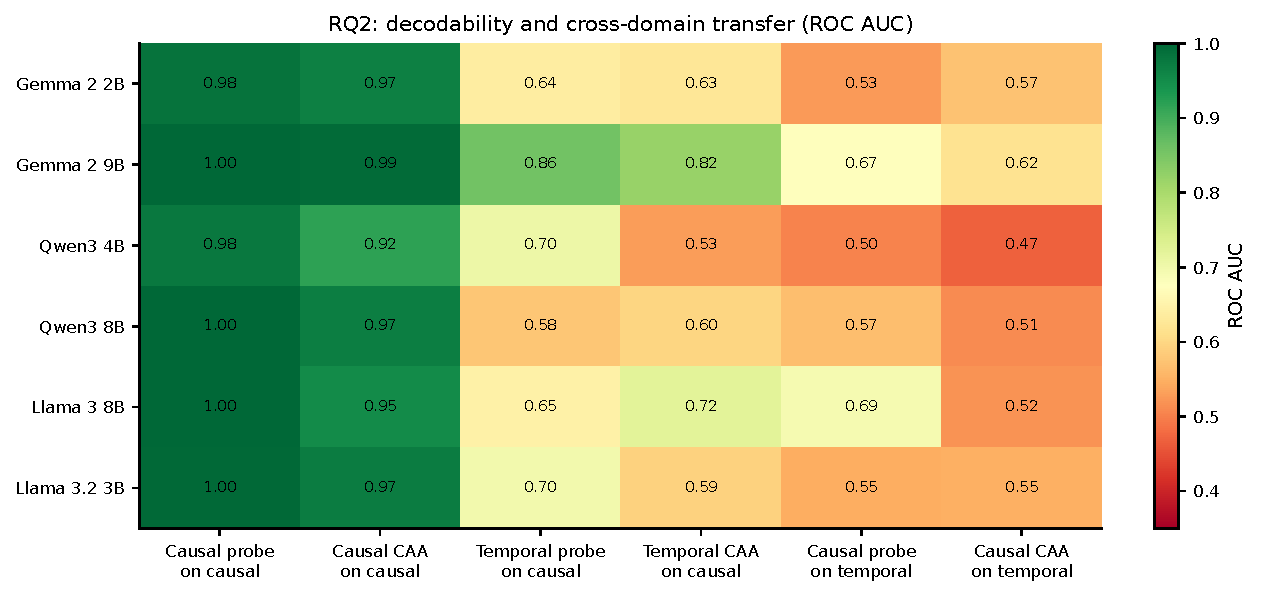
\includegraphics[width=.92\textwidth]{figures/rq1_decodability_transfer.pdf}
\caption{Development-selected probe and CAA ROC-AUC in domain and under causal--temporal transfer. All layers are frozen before test evaluation.}
\label{fig:rq2-transfer}
\end{figure*}

High representational discrimination does not guarantee calibrated behavior. Table~\ref{tab:rq1-direct} shows strong direct rank discrimination for Qwen3 4B and 8B but much weaker discrimination for Gemma 2 2B, Llama 3 8B, and Llama 3.2 3B. Fixed-threshold analyses additionally place the latter three near chance in balanced accuracy. Some of these failures are decision-level collapses: Gemma 2 2B predicts positive on 99.7\% of items under Yes-or-No but on 0\% under No-or-Yes, while its AUC remains 0.608 and 0.654, respectively. Llama 3 8B likewise shifts from a 93.7\% to an 11.7\% positive rate when answer order is reversed. Across models, the mean within-model balanced-accuracy range is 0.071 for Yes/No order and 0.046 for Likert anchor order. The rank-based metrics and fixed-threshold metrics thus diagnose different properties: encoded discrimination versus prompt-dependent decision calibration.

\subsection{RQ3: representations track external ratings more consistently than self-ratings}
Table~\ref{tab:rq3-pearson} reports primary row-level Pearson correlations. Probe correlations with a model's own order-averaged behavior are high for Qwen3 4B and 8B (0.785--0.905), moderate for Gemma 2 9B (0.572--0.593), and weak for Gemma 2 2B and both Llama models (0.139--0.262). CAA follows the same broad pattern but is usually weaker than the probe.

\begin{table*}[t]
\centering
\scriptsize
\resizebox{\textwidth}{!}{%
\begin{tabular}{lcccccc}
\toprule
Model & Probe--Y/N & Probe--Likert & Probe--Gemini & CAA--Y/N & CAA--Likert & CAA--Gemini \\
\midrule
Gemma 2 2B & $.199\pm.091$ & $.149\pm.094$ & $.829\pm.029$ & $.181\pm.100$ & $.104\pm.103$ & $.785\pm.032$ \\
Gemma 2 9B & $.572\pm.067$ & $.593\pm.057$ & $.922\pm.016$ & $.548\pm.076$ & $.567\pm.069$ & $.840\pm.026$ \\
Qwen3 4B & $.785\pm.034$ & $.806\pm.031$ & $.796\pm.036$ & $.656\pm.054$ & $.712\pm.040$ & $.692\pm.044$ \\
Qwen3 8B & $.879\pm.022$ & $.905\pm.015$ & $.889\pm.022$ & $.765\pm.034$ & $.793\pm.034$ & $.774\pm.041$ \\
Llama 3 8B & $.139\pm.081$ & $.204\pm.082$ & $.912\pm.014$ & $.056\pm.091$ & $.244\pm.089$ & $.761\pm.038$ \\
Llama 3.2 3B & $.239\pm.080$ & $.262\pm.077$ & $.871\pm.024$ & $.245\pm.087$ & $.219\pm.093$ & $.798\pm.031$ \\
\bottomrule
\end{tabular}}
\caption{Row-level Pearson correlations, shown as estimate $\pm$ half-width of the pair-clustered 95\% bootstrap interval. Y/N and Likert targets are item-level order averages.}
\label{tab:rq3-pearson}
\end{table*}

In contrast, probe--Gemini correlations range from 0.796 to 0.922, including 0.829 for Gemma 2 2B, 0.912 for Llama 3 8B, and 0.871 for Llama 3.2 3B. These models therefore contain a linearly accessible ordering that agrees with the external graded judgment even when their own final prompted decisions are poorly calibrated. This dissociation argues against interpreting low behavioral balanced accuracy as absence of causal information.

Spearman correlations reproduce the row-level pattern. Pair-difference correlations are considerably smaller: the largest probe Pearson value is 0.38 for Qwen3 4B and 8B, while most Gemini pair-difference correlations are near zero. The strong row-level association is therefore driven mainly by between-item ordering, not by covariation in the magnitude of each critical-minus-control shift. This distinction limits the claim: representations align with graded item plausibility, but do not robustly predict fine-grained paired effect sizes.

\subsection{RQ4: probe-relative failure prediction transfers unevenly}
The prompt-conditioned failure probe is evaluated on 1,200 held-out observations per model. Five of the six models transfer above chance, with balanced accuracies from 0.680 to 0.903 (Table~\ref{tab:rq4-probe}). Gemma 2 2B and Llama 3 8B are strongest at 0.903 and 0.897 balanced accuracy, respectively, and attain macro one-vs-rest AUC above 0.96. Qwen3 8B is the exception: its high overall accuracy (0.917) reflects the dominant correct class, while its balanced accuracy is 0.497 and its post-hoc recall is 0.390. Thus, high causal discrimination in RQ2 does not guarantee that a model's decision failures occupy a stable, linearly transferable state.

\begin{table}[t]
\centering
\small
\resizebox{\columnwidth}{!}{%
\begin{tabular}{lrrrrrrrr}
\toprule
Model & Layer & BAcc & Acc. & AUC & Supp. & Post-hoc & Correct \\
\midrule
Gemma 2 2B   & 17 & .90 & .89 & .96 & .92 & .93 & .86 \\
Gemma 2 9B   & 26 & .78 & .85 & .93 & .88 & .60 & .84 \\
Qwen3 4B     & 28 & .68 & .78 & .84 & .73 & .49 & .81 \\
Qwen3 8B     & 34 & .50 & .92 & .86 & .14 & .39 & .96 \\
Llama 3.2 3B & 13 & .84 & .83 & .93 & .89 & .86 & .78 \\
Llama 3 8B   & 17 & .90 & .88 & .96 & .95 & .90 & .84 \\
\bottomrule
\end{tabular}}
\caption{Frozen three-way probe-relative failure-probe performance on held-out items. Accuracy uses the probe's three-class argmax prediction, without a threshold. AUC is macro one-vs-rest ROC-AUC; the rightmost three columns are class recalls.}
\label{tab:rq4-probe}
\end{table}

\subsection{RQ4: targeted interventions improve some endpoints}
Classifier-gated steering has strongly model- and endpoint-dependent effects (Figure~\ref{fig:rq4-intervention}). The largest Yes/No AUC gains occur for Gemma 2 9B, from 0.830 to 0.985 ($\Delta=0.155$), and Llama 3 8B, from 0.589 to 0.712 ($\Delta=0.123$). Gemma 2 9B Likert improves from 0.866 to 0.919, and Llama 3.2 3B Likert improves from 0.636 to 0.710. The Qwen models show smaller positive changes. Effects need not improve every endpoint: Llama 3 8B Likert falls from 0.567 to 0.473, while Gemma 2 2B changes little.

\begin{figure*}[t]
\centering
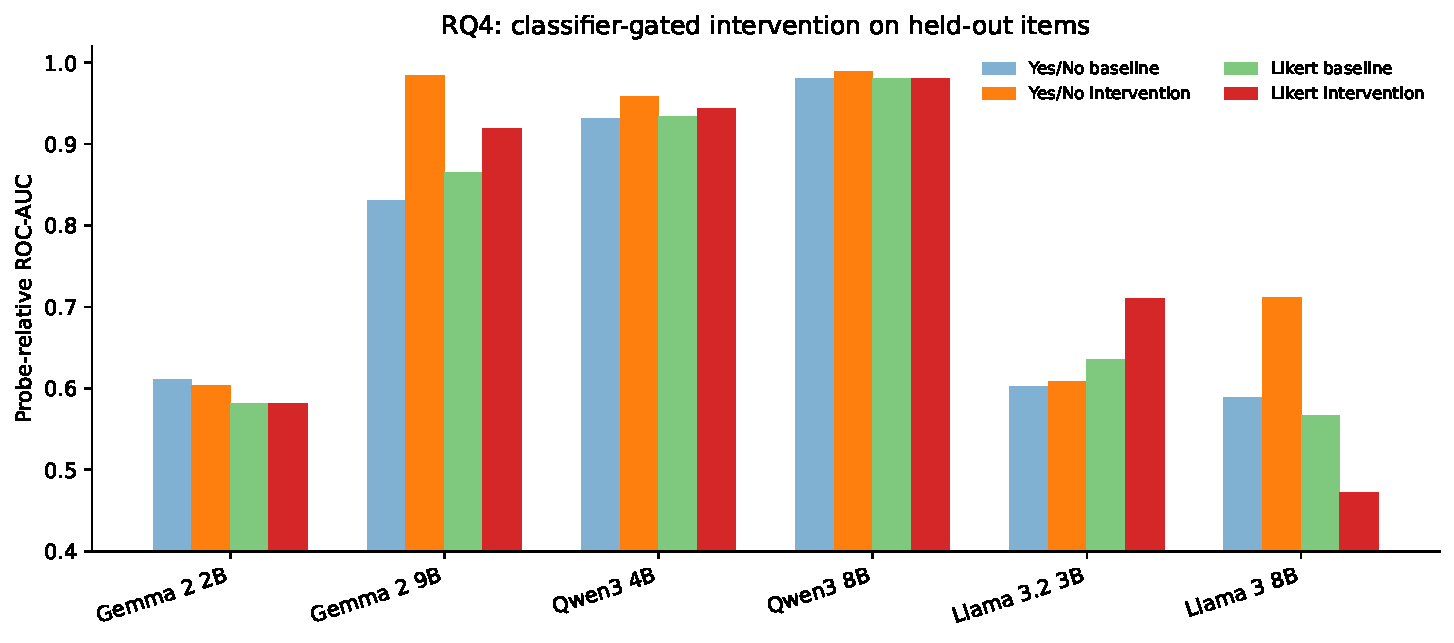
\includegraphics[width=.94\textwidth]{figures/rq4_intervention_auc.pdf}
\caption{Baseline and classifier-gated intervention ROC-AUC against the frozen causal-probe reference on held-out items. Values average the two prompt orders within each endpoint.}
\label{fig:rq4-intervention}
\end{figure*}

Development selection retains $\alpha=0$ when no positive penalized effect is supported, and some endpoint--failure combinations provide no estimable contrast vector. These null selections explain the unchanged aggregate cells. They are informative outcomes under this protocol, not evidence that no nonlinear or more localized intervention could work. More generally, subtracting a failure contrast and observing a predicted output shift provides causal evidence that the selected residual component influences the answer, but does not establish that the vector isolates the full mechanism of causal implication.


\section*{Limitations}
Linear decodability does not identify a unique causal mechanism. The intervention vectors contrast naturally occurring error and matched-correct states and can therefore contain correlated features unrelated to the targeted failure. Prompt-order effects also show that failure labels partly depend on the measurement interface.

\bibliographystyle{plainnat}
\ifcompiledfromparent
  \bibliography{workshop/custom}
\else
  \bibliography{custom}
\fi

\appendix
\section{Probe-relative failure categories}
\label{app:failure-grid}

Figure~\ref{fig:failure-grid} summarizes the probe-relative labels used in RQ4. The frozen causal probe supplies the reference decision by thresholding its raw logit at zero. The prompted model decision is obtained from either the normalized Yes/No probability or normalized probabilistic Likert score at threshold 0.5; ties are negative. Labels are assigned separately to every item--prompt observation.

\begin{figure*}[t]
\centering
\large
\renewcommand{\arraystretch}{2.2}
\setlength{\tabcolsep}{16pt}
\resizebox{.92\textwidth}{!}{%
\begin{tabular}{c|c|c}
& \multicolumn{2}{c}{\textbf{Model output}} \\
\textbf{Causal-probe decision} & \textbf{Positive} & \textbf{Negative} \\
\hline
\textbf{Positive}
& \shortstack{\textbf{True positive}\\Probe--output agreement}
& \shortstack{\textbf{Suppression}\\Probe positive, output negative} \\
\hline
\textbf{Negative}
& \shortstack{\textbf{Post-hoc attribution}\\Probe negative, output positive}
& \shortstack{\textbf{True negative}\\Probe--output agreement} \\
\hline
\end{tabular}}
\caption{Visual definition of the probe-relative RQ4 categories. \emph{True positive} and \emph{true negative} denote agreement with the frozen causal-probe decision; they do not assert agreement with dataset ground truth.}
\label{fig:failure-grid}
\end{figure*}


\newpage
\section*{NeurIPS Paper Checklist}

\begin{enumerate}

\item {\bf Claims}
    \item[] Question: Do the main claims made in the abstract and introduction accurately reflect the paper's contributions and scope?
    \item[] Answer: \answerTODO{} % Replace by \answerYes{}, \answerNo{}, or \answerNA{}.
    \item[] Justification: \justificationTODO{}
    \item[] Guidelines:
    \begin{itemize}
        \item The answer \answerNA{} means that the abstract and introduction do not include the claims made in the paper.
        \item The abstract and/or introduction should clearly state the claims made, including the contributions made in the paper and important assumptions and limitations. A \answerNo{} or \answerNA{} answer to this question will not be perceived well by the reviewers. 
        \item The claims made should match theoretical and experimental results, and reflect how much the results can be expected to generalize to other settings. 
        \item It is fine to include aspirational goals as motivation as long as it is clear that these goals are not attained by the paper. 
    \end{itemize}

\item {\bf Limitations}
    \item[] Question: Does the paper discuss the limitations of the work performed by the authors?
    \item[] Answer: \answerTODO{} % Replace by \answerYes{}, \answerNo{}, or \answerNA{}.
    \item[] Justification: \justificationTODO{}
    \item[] Guidelines:
    \begin{itemize}
        \item The answer \answerNA{} means that the paper has no limitation while the answer \answerNo{} means that the paper has limitations, but those are not discussed in the paper. 
        \item The authors are encouraged to create a separate ``Limitations'' section in their paper.
        \item The paper should point out any strong assumptions and how robust the results are to violations of these assumptions (e.g., independence assumptions, noiseless settings, model well-specification, asymptotic approximations only holding locally). The authors should reflect on how these assumptions might be violated in practice and what the implications would be.
        \item The authors should reflect on the scope of the claims made, e.g., if the approach was only tested on a few datasets or with a few runs. In general, empirical results often depend on implicit assumptions, which should be articulated.
        \item The authors should reflect on the factors that influence the performance of the approach. For example, a facial recognition algorithm may perform poorly when image resolution is low or images are taken in low lighting. Or a speech-to-text system might not be used reliably to provide closed captions for online lectures because it fails to handle technical jargon.
        \item The authors should discuss the computational efficiency of the proposed algorithms and how they scale with dataset size.
        \item If applicable, the authors should discuss possible limitations of their approach to address problems of privacy and fairness.
        \item While the authors might fear that complete honesty about limitations might be used by reviewers as grounds for rejection, a worse outcome might be that reviewers discover limitations that aren't acknowledged in the paper. The authors should use their best judgment and recognize that individual actions in favor of transparency play an important role in developing norms that preserve the integrity of the community. Reviewers will be specifically instructed to not penalize honesty concerning limitations.
    \end{itemize}

\item {\bf Theory assumptions and proofs}
    \item[] Question: For each theoretical result, does the paper provide the full set of assumptions and a complete (and correct) proof?
    \item[] Answer: \answerTODO{} % Replace by \answerYes{}, \answerNo{}, or \answerNA{}.
    \item[] Justification: \justificationTODO{}
    \item[] Guidelines:
    \begin{itemize}
        \item The answer \answerNA{} means that the paper does not include theoretical results. 
        \item All the theorems, formulas, and proofs in the paper should be numbered and cross-referenced.
        \item All assumptions should be clearly stated or referenced in the statement of any theorems.
        \item The proofs can either appear in the main paper or the supplemental material, but if they appear in the supplemental material, the authors are encouraged to provide a short proof sketch to provide intuition. 
        \item Inversely, any informal proof provided in the core of the paper should be complemented by formal proofs provided in appendix or supplemental material.
        \item Theorems and Lemmas that the proof relies upon should be properly referenced. 
    \end{itemize}

    \item {\bf Experimental result reproducibility}
    \item[] Question: Does the paper fully disclose all the information needed to reproduce the main experimental results of the paper to the extent that it affects the main claims and/or conclusions of the paper (regardless of whether the code and data are provided or not)?
    \item[] Answer: \answerTODO{} % Replace by \answerYes{}, \answerNo{}, or \answerNA{}.
    \item[] Justification: \justificationTODO{}
    \item[] Guidelines:
    \begin{itemize}
        \item The answer \answerNA{} means that the paper does not include experiments.
        \item If the paper includes experiments, a \answerNo{} answer to this question will not be perceived well by the reviewers: Making the paper reproducible is important, regardless of whether the code and data are provided or not.
        \item If the contribution is a dataset and\slash or model, the authors should describe the steps taken to make their results reproducible or verifiable. 
        \item Depending on the contribution, reproducibility can be accomplished in various ways. For example, if the contribution is a novel architecture, describing the architecture fully might suffice, or if the contribution is a specific model and empirical evaluation, it may be necessary to either make it possible for others to replicate the model with the same dataset, or provide access to the model. In general. releasing code and data is often one good way to accomplish this, but reproducibility can also be provided via detailed instructions for how to replicate the results, access to a hosted model (e.g., in the case of a large language model), releasing of a model checkpoint, or other means that are appropriate to the research performed.
        \item While NeurIPS does not require releasing code, the conference does require all submissions to provide some reasonable avenue for reproducibility, which may depend on the nature of the contribution. For example
        \begin{enumerate}
            \item If the contribution is primarily a new algorithm, the paper should make it clear how to reproduce that algorithm.
            \item If the contribution is primarily a new model architecture, the paper should describe the architecture clearly and fully.
            \item If the contribution is a new model (e.g., a large language model), then there should either be a way to access this model for reproducing the results or a way to reproduce the model (e.g., with an open-source dataset or instructions for how to construct the dataset).
            \item We recognize that reproducibility may be tricky in some cases, in which case authors are welcome to describe the particular way they provide for reproducibility. In the case of closed-source models, it may be that access to the model is limited in some way (e.g., to registered users), but it should be possible for other researchers to have some path to reproducing or verifying the results.
        \end{enumerate}
    \end{itemize}


\item {\bf Open access to data and code}
    \item[] Question: Does the paper provide open access to the data and code, with sufficient instructions to faithfully reproduce the main experimental results, as described in supplemental material?
    \item[] Answer: \answerTODO{} % Replace by \answerYes{}, \answerNo{}, or \answerNA{}.
    \item[] Justification: \justificationTODO{}
    \item[] Guidelines:
    \begin{itemize}
        \item The answer \answerNA{} means that paper does not include experiments requiring code.
        \item Please see the NeurIPS code and data submission guidelines (\url{https://neurips.cc/public/guides/CodeSubmissionPolicy}) for more details.
        \item While we encourage the release of code and data, we understand that this might not be possible, so \answerNo{} is an acceptable answer. Papers cannot be rejected simply for not including code, unless this is central to the contribution (e.g., for a new open-source benchmark).
        \item The instructions should contain the exact command and environment needed to run to reproduce the results. See the NeurIPS code and data submission guidelines (\url{https://neurips.cc/public/guides/CodeSubmissionPolicy}) for more details.
        \item The authors should provide instructions on data access and preparation, including how to access the raw data, preprocessed data, intermediate data, and generated data, etc.
        \item The authors should provide scripts to reproduce all experimental results for the new proposed method and baselines. If only a subset of experiments are reproducible, they should state which ones are omitted from the script and why.
        \item At submission time, to preserve anonymity, the authors should release anonymized versions (if applicable).
        \item Providing as much information as possible in supplemental material (appended to the paper) is recommended, but including URLs to data and code is permitted.
    \end{itemize}


\item {\bf Experimental setting/details}
    \item[] Question: Does the paper specify all the training and test details (e.g., data splits, hyperparameters, how they were chosen, type of optimizer) necessary to understand the results?
    \item[] Answer: \answerTODO{} % Replace by \answerYes{}, \answerNo{}, or \answerNA{}.
    \item[] Justification: \justificationTODO{}
    \item[] Guidelines:
    \begin{itemize}
        \item The answer \answerNA{} means that the paper does not include experiments.
        \item The experimental setting should be presented in the core of the paper to a level of detail that is necessary to appreciate the results and make sense of them.
        \item The full details can be provided either with the code, in appendix, or as supplemental material.
    \end{itemize}

\item {\bf Experiment statistical significance}
    \item[] Question: Does the paper report error bars suitably and correctly defined or other appropriate information about the statistical significance of the experiments?
    \item[] Answer: \answerTODO{} % Replace by \answerYes{}, \answerNo{}, or \answerNA{}.
    \item[] Justification: \justificationTODO{}
    \item[] Guidelines:
    \begin{itemize}
        \item The answer \answerNA{} means that the paper does not include experiments.
        \item The authors should answer \answerYes{} if the results are accompanied by error bars, confidence intervals, or statistical significance tests, at least for the experiments that support the main claims of the paper.
        \item The factors of variability that the error bars are capturing should be clearly stated (for example, train/test split, initialization, random drawing of some parameter, or overall run with given experimental conditions).
        \item The method for calculating the error bars should be explained (closed form formula, call to a library function, bootstrap, etc.)
        \item The assumptions made should be given (e.g., Normally distributed errors).
        \item It should be clear whether the error bar is the standard deviation or the standard error of the mean.
        \item It is OK to report 1-sigma error bars, but one should state it. The authors should preferably report a 2-sigma error bar than state that they have a 96\% CI, if the hypothesis of Normality of errors is not verified.
        \item For asymmetric distributions, the authors should be careful not to show in tables or figures symmetric error bars that would yield results that are out of range (e.g., negative error rates).
        \item If error bars are reported in tables or plots, the authors should explain in the text how they were calculated and reference the corresponding figures or tables in the text.
    \end{itemize}

\item {\bf Experiments compute resources}
    \item[] Question: For each experiment, does the paper provide sufficient information on the computer resources (type of compute workers, memory, time of execution) needed to reproduce the experiments?
    \item[] Answer: \answerTODO{} % Replace by \answerYes{}, \answerNo{}, or \answerNA{}.
    \item[] Justification: \justificationTODO{}
    \item[] Guidelines:
    \begin{itemize}
        \item The answer \answerNA{} means that the paper does not include experiments.
        \item The paper should indicate the type of compute workers CPU or GPU, internal cluster, or cloud provider, including relevant memory and storage.
        \item The paper should provide the amount of compute required for each of the individual experimental runs as well as estimate the total compute. 
        \item The paper should disclose whether the full research project required more compute than the experiments reported in the paper (e.g., preliminary or failed experiments that didn't make it into the paper). 
    \end{itemize}
    
\item {\bf Code of ethics}
    \item[] Question: Does the research conducted in the paper conform, in every respect, with the NeurIPS Code of Ethics \url{https://neurips.cc/public/EthicsGuidelines}?
    \item[] Answer: \answerTODO{} % Replace by \answerYes{}, \answerNo{}, or \answerNA{}.
    \item[] Justification: \justificationTODO{}
    \item[] Guidelines:
    \begin{itemize}
        \item The answer \answerNA{} means that the authors have not reviewed the NeurIPS Code of Ethics.
        \item If the authors answer \answerNo, they should explain the special circumstances that require a deviation from the Code of Ethics.
        \item The authors should make sure to preserve anonymity (e.g., if there is a special consideration due to laws or regulations in their jurisdiction).
    \end{itemize}


\item {\bf Broader impacts}
    \item[] Question: Does the paper discuss both potential positive societal impacts and negative societal impacts of the work performed?
    \item[] Answer: \answerTODO{} % Replace by \answerYes{}, \answerNo{}, or \answerNA{}.
    \item[] Justification: \justificationTODO{}
    \item[] Guidelines:
    \begin{itemize}
        \item The answer \answerNA{} means that there is no societal impact of the work performed.
        \item If the authors answer \answerNA{} or \answerNo, they should explain why their work has no societal impact or why the paper does not address societal impact.
        \item Examples of negative societal impacts include potential malicious or unintended uses (e.g., disinformation, generating fake profiles, surveillance), fairness considerations (e.g., deployment of technologies that could make decisions that unfairly impact specific groups), privacy considerations, and security considerations.
        \item The conference expects that many papers will be foundational research and not tied to particular applications, let alone deployments. However, if there is a direct path to any negative applications, the authors should point it out. For example, it is legitimate to point out that an improvement in the quality of generative models could be used to generate Deepfakes for disinformation. On the other hand, it is not needed to point out that a generic algorithm for optimizing neural networks could enable people to train models that generate Deepfakes faster.
        \item The authors should consider possible harms that could arise when the technology is being used as intended and functioning correctly, harms that could arise when the technology is being used as intended but gives incorrect results, and harms following from (intentional or unintentional) misuse of the technology.
        \item If there are negative societal impacts, the authors could also discuss possible mitigation strategies (e.g., gated release of models, providing defenses in addition to attacks, mechanisms for monitoring misuse, mechanisms to monitor how a system learns from feedback over time, improving the efficiency and accessibility of ML).
    \end{itemize}
    
\item {\bf Safeguards}
    \item[] Question: Does the paper describe safeguards that have been put in place for responsible release of data or models that have a high risk for misuse (e.g., pre-trained language models, image generators, or scraped datasets)?
    \item[] Answer: \answerTODO{} % Replace by \answerYes{}, \answerNo{}, or \answerNA{}.
    \item[] Justification: \justificationTODO{}
    \item[] Guidelines:
    \begin{itemize}
        \item The answer \answerNA{} means that the paper poses no such risks.
        \item Released models that have a high risk for misuse or dual-use should be released with necessary safeguards to allow for controlled use of the model, for example by requiring that users adhere to usage guidelines or restrictions to access the model or implementing safety filters. 
        \item Datasets that have been scraped from the Internet could pose safety risks. The authors should describe how they avoided releasing unsafe images.
        \item We recognize that providing effective safeguards is challenging, and many papers do not require this, but we encourage authors to take this into account and make a best faith effort.
    \end{itemize}

\item {\bf Licenses for existing assets}
    \item[] Question: Are the creators or original owners of assets (e.g., code, data, models), used in the paper, properly credited and are the license and terms of use explicitly mentioned and properly respected?
    \item[] Answer: \answerTODO{} % Replace by \answerYes{}, \answerNo{}, or \answerNA{}.
    \item[] Justification: \justificationTODO{}
    \item[] Guidelines:
    \begin{itemize}
        \item The answer \answerNA{} means that the paper does not use existing assets.
        \item The authors should cite the original paper that produced the code package or dataset.
        \item The authors should state which version of the asset is used and, if possible, include a URL.
        \item The name of the license (e.g., CC-BY 4.0) should be included for each asset.
        \item For scraped data from a particular source (e.g., website), the copyright and terms of service of that source should be provided.
        \item If assets are released, the license, copyright information, and terms of use in the package should be provided. For popular datasets, \url{paperswithcode.com/datasets} has curated licenses for some datasets. Their licensing guide can help determine the license of a dataset.
        \item For existing datasets that are re-packaged, both the original license and the license of the derived asset (if it has changed) should be provided.
        \item If this information is not available online, the authors are encouraged to reach out to the asset's creators.
    \end{itemize}

\item {\bf New assets}
    \item[] Question: Are new assets introduced in the paper well documented and is the documentation provided alongside the assets?
    \item[] Answer: \answerTODO{} % Replace by \answerYes{}, \answerNo{}, or \answerNA{}.
    \item[] Justification: \justificationTODO{}
    \item[] Guidelines:
    \begin{itemize}
        \item The answer \answerNA{} means that the paper does not release new assets.
        \item Researchers should communicate the details of the dataset\slash code\slash model as part of their submissions via structured templates. This includes details about training, license, limitations, etc. 
        \item The paper should discuss whether and how consent was obtained from people whose asset is used.
        \item At submission time, remember to anonymize your assets (if applicable). You can either create an anonymized URL or include an anonymized zip file.
    \end{itemize}

\item {\bf Crowdsourcing and research with human subjects}
    \item[] Question: For crowdsourcing experiments and research with human subjects, does the paper include the full text of instructions given to participants and screenshots, if applicable, as well as details about compensation (if any)? 
    \item[] Answer: \answerTODO{} % Replace by \answerYes{}, \answerNo{}, or \answerNA{}.
    \item[] Justification: \justificationTODO{}
    \item[] Guidelines:
    \begin{itemize}
        \item The answer \answerNA{} means that the paper does not involve crowdsourcing nor research with human subjects.
        \item Including this information in the supplemental material is fine, but if the main contribution of the paper involves human subjects, then as much detail as possible should be included in the main paper. 
        \item According to the NeurIPS Code of Ethics, workers involved in data collection, curation, or other labor should be paid at least the minimum wage in the country of the data collector. 
    \end{itemize}

\item {\bf Institutional review board (IRB) approvals or equivalent for research with human subjects}
    \item[] Question: Does the paper describe potential risks incurred by study participants, whether such risks were disclosed to the subjects, and whether Institutional Review Board (IRB) approvals (or an equivalent approval/review based on the requirements of your country or institution) were obtained?
    \item[] Answer: \answerTODO{} % Replace by \answerYes{}, \answerNo{}, or \answerNA{}.
    \item[] Justification: \justificationTODO{}
    \item[] Guidelines:
    \begin{itemize}
        \item The answer \answerNA{} means that the paper does not involve crowdsourcing nor research with human subjects.
        \item Depending on the country in which research is conducted, IRB approval (or equivalent) may be required for any human subjects research. If you obtained IRB approval, you should clearly state this in the paper. 
        \item We recognize that the procedures for this may vary significantly between institutions and locations, and we expect authors to adhere to the NeurIPS Code of Ethics and the guidelines for their institution. 
        \item For initial submissions, do not include any information that would break anonymity (if applicable), such as the institution conducting the review.
    \end{itemize}

\item {\bf Declaration of LLM usage}
    \item[] Question: Does the paper describe the usage of LLMs if it is an important, original, or non-standard component of the core methods in this research? Note that if the LLM is used only for writing, editing, or formatting purposes and does \emph{not} impact the core methodology, scientific rigor, or originality of the research, declaration is not required.
    %this research? 
    \item[] Answer: \answerTODO{} % Replace by \answerYes{}, \answerNo{}, or \answerNA{}.
    \item[] Justification: \justificationTODO{}
    \item[] Guidelines:
    \begin{itemize}
        \item The answer \answerNA{} means that the core method development in this research does not involve LLMs as any important, original, or non-standard components.
        \item Please refer to our LLM policy in the NeurIPS handbook for what should or should not be described.
    \end{itemize}

\end{enumerate}


\end{document}
